\documentclass[a4paper,11pt]{article}

%% We can use macros to avoid typing the same thing over and over
\newcommand{\token}[1]{\texttt{<#1>}}
\newcommand{\uC}{{$\mathrm{\mu}$}C }
 \usepackage{tikz}
 \usepackage{tikz-qtree}
 \usepackage{array}
\usepackage{amsmath}
\usepackage{multicol}
\usepackage{listings}
\usepackage{mips}
\usepackage{alltt}
\usepackage{hyperref}
\usepackage[lighttt]{lmodern}

%% Simple syntax highlighting for our RTL. Add more keywords here.
\lstset{language=[mips]Assembler,
  morekeywords={Procedure, ADD, SUB, MUL, DIV, LTEQ, LT, EQ, NE, GTEQ, GT, Mov,
    Not, Neg, Jump, Branch, Zero, NonZero, IntConst, GlobalAddress, Store, Load,
    BYTE, INT, Call, ArrayAddress}}

\title{Assignment 4: ICode Generation \\
       Compiler Design Project, 1DL420}
\author{Xiao Yang \and Magnus L{\aa}ng}
\date{\today}
\begin{document}
\maketitle

\section{Technique Issues}
\subsection{Control Flows}
	We translate \textbf{While Statements}, \textbf{If Statements},
    the binary operator \textbf{\&\& }, and \textbf{Return Statements}
    into \textit{control flow} in our RTL.
	\begin{itemize}
	\item \textbf{While Statement}
		\begin{lstlisting}
Jump while_cond
while_loop:
# instructions in the while loop
while_cond:
# instructions to evaluate the conditions
# and put the result into r
Branch while_loop, NonZero, r
		\end{lstlisting}

	\item \textbf{If Statement}
	\begin{lstlisting}
# instructions to evalution the conditions
# and put the result into r
Branch end_if, Zero, r
# instructions in the if statement
end_if:
	\end{lstlisting}

	\item \textbf{\&\& Operator}
	\begin{lstlisting}
# evaluate the LHS and put the result into r0
Branch andshortcircut, NonZero, r0
# evaluate the RHS
andshortcircut:
	\end{lstlisting}

	\item \textbf{Return Statement}
	\begin{lstlisting}
# evaluate the expression (if any), into some register rt.
# This is of course omitted if there is no return expression.
RV <- Mov rt
Jump procedure.exit
# All procedures end with an exit label:
procedure.exit:
	\end{lstlisting}
	\end{itemize}
\subsection{Variables}
\begin{itemize}
	\item \textbf{Local Variable}

      We allocate a \textit{register} for a local variable declaration.

      During the translation, we maintain a list of registers allocated for
      certain procedure. So when a reference to a local variable in the source
      code is encountered , the corresponding allocated register is used in RTL.

	\item \textbf{Global Variable}

      We generate a \textit{label} for a global variable declaration.

      We use the RTL instruction \textit{GlobalAddress} to fetch the address of
      a global variable. We then use RTL instruction \textit{Load} or
      \textit{Store} to load or store it's value, as appropriate.

	\item \textbf{Local Array}

      When a local array is declared, we allocate slots on the frame to store
      it. Thus, the frame size in RTL is the total length of the local arrays.

      Each time an array reference is encountered, we use \textit{ArrayAddress}
      to fetch the base address of the array.

	\item \textbf{Global Array}

      The same as global variables, when an declaration of global array is
      encountered, we generate a label for it.

      For reference resolution, the only difference is we use
      \textit{GlobalAddress} RTL instruction to fetch the base address of a
      global array.
	\end{itemize}

    A note about arrays: Becase we generate code that compute the \emph{value}
    of a reference when it is a scalar, but the \emph{address} when it is an
    array, we can uniformly generate code for all four types of array subscripts
    (local array, local pointer (\texttt{int[]}, f.ex.), global array, and
    global pointer) by just recursively calling
    \texttt{CodeGenerator.generateExpression} to get the base address.

\subsection{Expressions}
	An expression is flattened by generating corresponding instructions for AST
    subtree nodes in the bottom-up way. The intermediate result of a
    sub-expression is stored in temporary RTL registers and be operated on in
    the following expressions.

	For example, $m=x+y*3-z$ will have the following RTL code:
	\begin{lstlisting}
r8 <- IntConst 3
r7 <- MUL r3, r8
r6 <- ADD r2, r7
r5 <- SUB r6, r4
r1 <- Mov r5
	\end{lstlisting}

\subsection{Procedure}
For a procedure, we will generate the following code. We allocate temporaries for \textit{return value}, \textit{formals}, \textit{locals} and registers used for intermediate results.While space for local arrays is allocated on stack.
\begin{lstlisting}
Procedure procedure_name
    Argument count: #args
    Stack frame size: total_array_size
    Register types:
      RV: register_type
      R1: register_type
      ...

      Rn: register_type
    Instructions:
      ...
      exit_label

\end{lstlisting}

\section{RTL Design Rationale}
\paragraph{Why flat datatypes?}
Or, in other words, why did we redesign this:

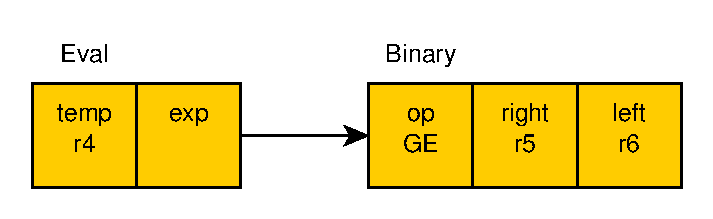
\includegraphics[scale=0.8]{bad}

to this:

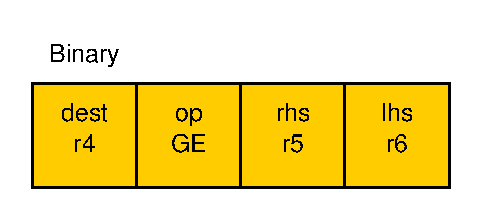
\includegraphics[scale=0.8]{good}

The answer is, we believe the \texttt{RtlExp} pattern facilitates minimal to no
code reuse, and complicates the instruction format, leading to a total of more,
less readable, code.

\paragraph{Why no distinction between locals and temporaries?} Because there is no
reason to. None of the subsequent processing needs to know what is a local and
what is a compiler-introduced temporary, so we cut the information away.

\paragraph{Why having regs $1,\, \dots,\, n$ be the $n$ formals?} Again, this is a
simplication of the format that for example makes it easier to identify what is
a reference to a formal (when required), without losing any expressiveness of
the language.

\paragraph{Why \texttt{\textbf{ArrayAddress}} instead of \texttt{FP}?} To simplify
adding additional offsets to the array area without generating additional
add-instructions or requiring data-flow optimisations to remove them. None of
the use-cases of FP that we considered is not covered by
\texttt{\textbf{ArrayAddress}}.

Also, unless special cases was added to the code generator, FP would have to be
stored in the stack frame together with all the other locals and temporaries (at
MIPS generation time, that is).

\paragraph{Why did we remove the empty interfaces?} There was no reason to keep
them. Since they were empty, they did not simplify anything, nor did they give
us any type guarantees for what instances might be.

We have no common interface (as in methods) of all our instructions except for
\texttt{toString}, which is provided by \texttt{Object} anyway.

\paragraph{But you could have added an enum of all the instruction types, and added
  a \texttt{getType} method to \texttt{RtlInsn}!} We considered that, but we
would have to combine that with either
\begin{itemize}
\item casts to the subtypes, which we needed anyway.
\item adding methods to \texttt{RtlInsn} that are only supported by a subset of
  instructions, which is terrible because incorrect assumptions about which
  methods are supported won't be caught by the type system.
\end{itemize}

\newpage
\appendix
% Puts the Appendix [letter] in all headings, and not just section headings,
% disabled for now
%% \renewcommand\thesection{Appendix \Alph{section}} %% Add the word ``Appendix'' to the numbering

\section{RTL Documentation}
This documentation is also distributed with the source code, in the
\path{doc/RTL.md} file.

%% Autogenerated from doc/RTL.md with ``kramdown'' tool, do not manually edit.
%% Autogenerated from doc/RTL.md with ``kramdown'' tool, do not manually edit.
\hypertarget{rtl}{}\label{rtl}

RTL operates on a register machine with an infinite amount of
registers. The registers are identified by integer numbers starting
with zero. Register zero is reserved for the return value of the
current procedure. Registers 1 through \emph{n} are the parameters to the
current \emph{n}-ary fuction.

All registers are associated with a type, described by the \emph{RtlType}
enumeration, having one of the following values.

\begin{verbatim}Int, Byte
\end{verbatim}

The size of an {\tt Int} is 4 bytes.

In addition to the registers, each procedure has a certain, specified
per procedure, number of bytes of stack space available for use. The
code aquires the address to this stack space using the {\tt ArrayAddress}
instruction.

\subsection{Instructions}\hypertarget{instructions}{}\label{instructions}

These are the available instructions in the RTL.

\subsubsection{Binary}\hypertarget{binary}{}\label{binary}

\begin{verbatim}Binary(Dest, BinOp, Lhs, Rhs)
\end{verbatim}

Computes a binary instruction that acts on two registers \emph{Lhs} and
\emph{Rhs}, and puts the result in a third register \emph{Dest}.

The \emph{BinOp} enumeration can have the following values.

\begin{verbatim}Add, Sub, Mul, Div, Gt, Lt, GtEq, LtEq, Eq, Ne
\end{verbatim}

The instruction is sometimes pretty-printed as

\begin{verbatim}Dest <- BinOp Lhs, Rhs
\end{verbatim}

\subsubsection{Unary}\hypertarget{unary}{}\label{unary}

Another instruction is {\tt Unary}:

\begin{verbatim}Unary(Dest, UnOp, Arg)
\end{verbatim}

Computes a unary operation that acts on a register \emph{Arg} and puts the
result in a register \emph{Dest}.

The \emph{UnOp} enumeration can have the following values.

\begin{verbatim}Not, Neg, Mov
\end{verbatim}

The instruction is sometimes pretty-printed as

\begin{verbatim}Dest <- UnOp Arg
\end{verbatim}

\subsubsection{Load}\hypertarget{load}{}\label{load}

The {\tt Load} instruction loads a value of type \emph{RtlType} from a memory
address stored in a register \emph{Addr} and writes the loaded value into
register \emph{Dest}.

\begin{verbatim}Load(Dest, RtlType, Addr)
\end{verbatim}

The instruction is sometimes pretty-printed as

\begin{verbatim}Dest <- Load RtlType Addr
\end{verbatim}

\subsubsection{Store}\hypertarget{store}{}\label{store}

The {\tt Store} instruction writes a value of type \emph{RtlType} stored in a
register \emph{Val} to a memory addres stored in register \emph{Addr}.

\begin{verbatim}Store(Addr, RtlType, Val)
\end{verbatim}

The instruction is sometimes pretty-printed as

\begin{verbatim}Addr <- Store RtlType Val
\end{verbatim}

\subsubsection{ArrayAddress}\hypertarget{arrayaddress}{}\label{arrayaddress}

The {\tt ArrayAddress} instruction computes a memory address that is
\emph{Offset} bytes after the memory location in the stack frame where
array locals are stored into a register \emph{Dest}. Note that \emph{Offset} is
an non-negative integer constant.

\begin{verbatim}ArrayAddress(Dest, Offset)
\end{verbatim}

The instruction is sometimes pretty-printed as

\begin{verbatim}Dest <- ArrayAddress Offset
\end{verbatim}

\subsubsection{GlobalAddress}\hypertarget{globaladdress}{}\label{globaladdress}

The {\tt GlobalAddress} instruction loads the memory address of a global
variable or constant with name \emph{Name} into a register \emph{Dest}.

\begin{verbatim}GlobalAddress(Dest, Name)
\end{verbatim}

The instruction is sometimes pretty-printed as

\begin{verbatim}Dest <- GlobalAddress Name
\end{verbatim}

\subsubsection{IntConst}\hypertarget{intconst}{}\label{intconst}

The {\tt IntConst} instruction loads an integer constant \emph{Const} into a
register \emph{Dest}.

\begin{verbatim}IntConst(Dest, Const)
\end{verbatim}

The instruction is sometimes pretty-printed as

\begin{verbatim}Dest <- IntConst Const
\end{verbatim}

\subsubsection{Label}\hypertarget{label}{}\label{label}

The {\tt Label} instruction has no side effects, but defines a location in
the program code that is identified by a string \emph{name}, and may be the
target of control flow instructions. The name must be unique in the
entire program, and may not clash with the names of functions or
global variables.

\begin{verbatim}Label(Name)
\end{verbatim}

The instruction is sometimes pretty-printed as

\begin{verbatim}Name:
\end{verbatim}

\subsubsection{Branch}\hypertarget{branch}{}\label{branch}

The {\tt Branch} instruction diverts control flow to after a {\tt Label}
instruction with name \emph{Name} in the same procedure based on the value
of the register \emph{Cond}.

\begin{verbatim}Branch(Name, Mode, Cond)
\end{verbatim}

The \emph{Mode} enumeration defines what values of the register \emph{Cond} that
causes the control flow to be diverted.

\begin{verbatim}Zero, NonZero
\end{verbatim}

The instruction is sometimes prettyprinted as

\begin{verbatim}Branch Name, Mode, Cond
\end{verbatim}

\subsubsection{Jump}\hypertarget{jump}{}\label{jump}

The {\tt Jump} instruction unconditinally transfers control flow to after a
{\tt Label} instructiom with name \emph{Name} in the same procedure.

\begin{verbatim}Jump(Name)
\end{verbatim}

The instruction is sometimes prettyprinted as

\begin{verbatim}Jump Name
\end{verbatim}

\subsubsection{Call}\hypertarget{call}{}\label{call}

The {\tt Call} instruction calls another procedure with the name \emph{Name},
sending the values of the registers \emph{Args} as arguments, placing the
return value in register \emph{Dest}.

\begin{verbatim}Call(Dest, Name, Args)
\end{verbatim}

The \emph{Dest} parameter may be -1, signifying that the return value (if
any) should be discarded. In this form, the instruction may be
constructed as

\begin{verbatim}Call(Name, Args)
\end{verbatim}

The instruction is sometimes prettyprinted as

\begin{verbatim}Dest <- Call Name [Arg [, Arg...]]

Call Name [Arg [, Arg...]]
\end{verbatim}


\section{Sample RTL for Test Files}
This is the RTL output from compiling the following programs.

\subsection{\texttt{quiet/lexer/l05.c}} \lstinputlisting{l05.rtl}
\subsection{\texttt{quiet/rtl/r01.c}}   \lstinputlisting{r01.rtl}
\subsection{\texttt{quiet/rtl/r02.c}}   \lstinputlisting{r02.rtl}
\subsection{\texttt{quiet/rtl/r03.c}}   \lstinputlisting{r03.rtl}
\subsection{\texttt{quiet/rtl/r04.c}}   \lstinputlisting{r04.rtl}
\subsection{\texttt{quiet/rtl/r05.c}}   \lstinputlisting{r05.rtl}

\end{document}
